\documentclass[a4paper, 11pt]{article}

\usepackage[utf8]{inputenc}
\usepackage[T1]{fontenc}
\usepackage{lmodern}
\usepackage{graphicx}
\usepackage[french]{babel}
\usepackage{geometry}
\geometry{left=2cm, right=2cm}

\usepackage{amsmath}
\usepackage{listings}
\usepackage{multicol}

\title{Campagne de Simulation}
\author{\textbf{Sorbonne Université} \\
	\textbf{Sciences Sorbonne Université} \\
	\textbf{Master informatique: RES} \\
	\textbf{PROGRES} \\ \\
	\texttt{Adrien Koumgang Tegantchouang 21109170}}
\date{\today}

\begin{document}
	\maketitle
	
	\newpage
	
	\tableofcontents
	
	\newpage
	
	\section{Présentation du projet}

		\subsection{Introduction}

			Le but de ce projet est d'utiliser un simulateur fourni pour mener une campagne de simulation: exécuter le simulateur avec de nombreux paramètres différents, collecter et manipuler les données produites par le simulateur, obtenir des graphiques résumant l'impact des paramètres suivis sur les indicateurs choisis.

			Ce simulateur est écrit en Java et modélise la propagation d'un virus dans une population. Il est fournit sous la forme d'un fichier Virus.jar qui intègre toutes les bibliothèques nécessaires. On peut lancer le simulateur avec les paramètres par défaut avec la commande (Java doit etre installé sur la machine qui exécute):

			```
			java -jar Virus.jar
			```

			Le code source du simulateur est fourni en annexe. Ce code source est fourni à titre indicatif pour comprendre la signification de chaque paramètre passé au simulateur.


		\subsection{La collecte des données expérimentales.}

			Réalisation en Python et en utilisant la bibliothèque `subprocess` un programme qui exécute plusieurs fois le simulateur avec les paramètres de simulation. Ces exécutions multiples sont utilisées pour obtenir des intervalles de confiance suffisants lors de la phase de visualisation des données expérimentales. Les résultats intermédiares sont stockés dans un ensemble de fichiers pour l'ensemble des simulations menées (pour un ensemble de paramètres donné).

			Dans un deuxième temps, on réalise en Python un programme qui exécute le simulateur en faisant varier un paramètre de la simulation, en réalisant plusieurs simulations pour chaque ensemble de paramètres. Les résultats intermédiaires sont stockés dans un ensemble de fichiers pour l'ensemble des simulations menées.


		\subsection{2. Manipulation des données expérimentales}

			A l'aide des fichiers produits précédemment, on réalise en Python et en utilisant les bibliothèques `numpy` et `pandas` un programme qui permette d'obtenir les informations suivantes:
			\begin{itemize}
				\item Quel est l'impact du nombre initial d'infectés sur:
				\begin{itemize}
					\item la durée de l'épidémie
					\item la proportion maximale de la population qui est infectée
					\item la distribution des multi-infections
				\end{itemize}
				
				\item Quel est l'impact du rayon de mobilité sur:
				\begin{itemize}
					\item la durée de l'épidémie
					\item la proportion de la population qui est infectée
					\item la distribution des multi-infections
				\end{itemize}
				
				\item Quel est l'impact de la proportion de vaccinés sur:
				\begin{itemize}
					\item la durée de l'épidémie
					\item la proportion de la population qui est infectée
					\item distribution des multi-infections
				\end{itemize}
				
				\item Quel est l'impact de l'efficacité vaccinale sur:
				\begin{itemize}
					\item la durée de l'épidémie
					\item la proportion de la population qui est infectée
					\item la distributuin des multi-infections
				\end{itemize}
				
				\item Quel est l'impact de la durée d'infection sur:
				\begin{itemize}
					\item la durée de l'épidémie
					\item la proportion de la population qui est infectée
					\item la distribution des multi-infections
				\end{itemize}
				
				\item Quel est l'impact de la durée de contagiosité sur:
				\begin{itemize}
					\item la durée de l'épidémie
					\item la proportion de la population qui est infectée
					\item la distribution des multi-infections
				\end{itemize}
				
				\item Quel est l'impact de la durée d'immunité sur:
				\begin{itemize}
					\item la durée de l'épidémie
					\item la proportion de la population qui est infectée
					\item la distribution des multi-infections
				\end{itemize}
				
				\item Quel est l'impact de la densité de population sur:
				\begin{itemize}
					\item la durée de l'épidémie
					\item la proportion de la population qui est infectée
					\item la distribution des multi-infections
				\end{itemize}
			\end{itemize}

			Les informations ainsi produites sont stockés dans plusieurs fichiers.


		\subsection{Tracer des données expérimentales}

			A l'aide des fichiers produits précédemment, on réalise en Python et en utilisant la bibliothèque `matplotlib` un programme qui produit des graphiques pertinents pour évaluer l'impact des paramètres suivis (nombre initial d'infectés, rayon de mobilité, proportion de vaccinés, efficacité vaccinale, durée de contagiosité, durée d'immunité, densité de population) sur les indicateurs sélectionnés (la durée de l'épidémie, la proportion de la population qui est infectée, la distribution des multi-infections). Les graphiques ainsi produits figures dans le rapport.


	\section{Présentation des parties principales de 'Simulation Campaign'}

		\subsection{La simulation}

			Elle se fait grace au code source simulator.py. Ce fichier python permet l'exécution d'un ensemble de simulation en fonction d'une variable passé en ligne de commande au programme et aussi d'un ensemble de paramètres, tout aussi passé en ligne de commande lors du lancement de l'exécution du programme. La syntax générale d'exécution du programme de simulation est la suivante:
			\begin{itemize}
				\item python3 -name\_var=name [-number\_of\_simulation=x]
				\item \hspace{4.51cm} [-variable\_value\_begin=x] 
				\item \hspace{4.51cm} [-variable\_value\_end=x] 
				\item \hspace{4.51cm} [-var\_value\_incremented=x]
				\item \hspace{4.51cm} [-other\_interest\_var=list\_var]
				\item \hspace{4.51cm} [-path\_save\_result=pathname]
			\end{itemize}
			

			\begin{itemize}
				\item name\_var: [name] name of the variable of interest
				\item [=0] for nb nodes
				\item [=1] for nb infected
				\item [=2] for travel distance
				\item [=3] for nb vaccinated
				\item [=4] for vaccine efficiency
				\item [=5] for infection period
				\item [=6] for contagion period
				\item [=7] for immune period
				\item [=x] number of simulations to do for each value of the variable of interest
				\item variable\_value\_begin:  [=x] initial value for variable simulation for the simulations
				\item variable\_value\_end:    [=x] final value for variable simulation for the simulations
				\item var\_value\_incremented: [=x] increment value for variable simulation
				\item other\_interest\_var:    [=list\_var] list of other parameters to switch to the simulator. ex: -stop\_all\_sane=1,-gui=0,-printout=2
				\item path\_save\_result:      [=pathname] path to directory where save file to result of the simulator
			\end{itemize}

			Ces informations peuvent être obtenu depuis le code source en l'exécutant sans arguments.

			Pour ce projet, nous nous sommes intéressés à 8 variables et créer des fichiers 'bash' pour chacune d'elle enfin d'y passer des paramètres exact pour leur simulation:
			
			\begin{itemize}
				\item contagion\_period (var\_contagion\_period\_simulation.sh):
				\begin{itemize}
					\item name\_var = 6
					\item nombre de simulations = 50
					\item valeur de début = 150
					\item valeur de fin = 300
					\item shift = 10
					\item paramètres à passer au simulateur: '-stop\_all\_sane=1, -gui=0, -printout=2'
					\item dossiers de sauvegardes des fichiers résultats des simulations : 'result\_simulations/contagion\_period'
				\end{itemize}
				
				\item immune\_period (var\_immune\_period\_simulation.sh):
				\begin{itemize}
					\item name\_var = 7
					\item nombre de simulations = 100
					\item valeur de début = 200
					\item valeur de fin = 400
					\item shift = 20
					\item paramètres à passer au simulateur: '-stop\_all\_sane=1, -gui=0, -printout=2'
					\item dossiers de sauvegardes des fichiers résultats des simulations : 'result\_simulations/immune\_period'
				\end{itemize}
				
				\item nb\_infected (var\_nb\_infected\_simulation.sh):
				\begin{itemize}
					\item name\_var = 1
					\item nombre de simulations = 100
					\item valeur de début = 1
					\item valeur de fin = 10
					\item shift = 1
					\item paramètres à passer au simulateur: '-stop\_all\_sane=1, -gui=0, -printout=2'
					\item dossiers de sauvegardes des fichiers résultats des simulations : 'result\_simulations/nb\_infected'
				\end{itemize}
				
				\item infection\_period (var\_infection\_period\_simulation.sh):
				\begin{itemize}
					\item name\_var = 5
					\item nombre de simulations = 100
					\item valeur de début = 50
					\item valeur de fin = 150
					\item shift = 10
					\item paramètres à passer au simulateur: '-stop\_all\_sane=1, -gui=0, -printout=2'
					\item dossiers de sauvegardes des fichiers résultats des simulations : 'result\_simulations/infection\_period'
				\end{itemize}
				
				\item nb\_nodes (var\_nb\_nodes\_simulation.sh):
				\begin{itemize}
					\item name\_var = 0
					\item nombre de simulations = 100
					\item valeur de début = 100
					\item valeur de fin = 150
					\item shift = 10
					\item paramètres à passer au simulateur: '-stop\_all\_sane=1, -gui=0, -printout=2'
					\item dossiers de sauvegardes des fichiers résultats des simulations : 'result\_simulations/nb\_nodes'
				\end{itemize}
				
				\item travel\_distance (var\_travel\_distance\_simulation.sh):
				\begin{itemize}
					\item name\_var = 2
					\item nombre de simulations = 100
					\item valeur de début = 150
					\item valeur de fin = 250
					\item shift = 10
					\item paramètres à passer au simulateur: '-stop\_all\_sane=1, -gui=0, -printout=2'
					\item dossiers de sauvegardes des fichiers résultats des simulations : 'result\_simulations/travel\_distance'
				\end{itemize}
				
				\item nb\_vaccinated (var\_nb\_vaccinated\_simulation.sh):
				\begin{itemize}
					\item name\_var = 3
					\item nombre de simulations = 100
					\item valeur de début = 0
					\item valeur de fin = 10
					\item shift = 1
					\item paramètres à passer au simulateur: '-stop\_all\_sane=1, -gui=0, -printout=2'
					\item dossiers de sauvegardes des fichiers résultats des simulations : 'result\_simulations/nb\_vaccinated'
				\end{itemize}
				
				\item vaccine\_efficiency (var\_vaccine\_efficiency\_simulation.sh):
				\begin{itemize}
					\item name\_var = 4
					\item nombre de simulations = 100
					\item valeur de début = 1
					\item valeur de fin = 10
					\item shift = 1
					\item paramètres à passer au simulateur: '-stop\_all\_sane=1, -gui=0, -printout=2'
					\item dossiers de sauvegardes des fichiers résultats des simulations : 'result\_simulations/vaccine\_efficiency'
				\end{itemize}
			\end{itemize}


			Le programme de simulation offre un feedback de 2 niveaux :
			\begin{itemize}
				\item le premier : il affiche les paramètres passés au simulateur
				\item le deuxième : pour chaque valeur de la variable de simulation, il indique à quelle simulation il se situe
			\end{itemize}

			Nous avons choisit d'implementer le simulateur de cette manière enfin de permettre la simulation précise d'une variable ainsi que de ses valeurs aux choix. (Ceci dû au tant que prend les simulations, cela nous a permit de lancer une simulation puis de l'arreter pour la relancer plus tard, donnant ainsi une grande flexibilité dans l'exécution des simulations)

		\subsection{L'analyse des simulations}

			Elle se fait grâce au code source analyse.py. Ici, l'analyse des fichiers résultats de la simulation se fait en parallèle pour chaque variable. Ainsi on a un thread qui s'occupe de l'analyse de chaque variable.

			L'analyse des fichiers est orienté principalement sur 3 points :
			\begin{itemize}
				\item Calcul de la durée de chaque simulation. Et elle se fait grâce à la fonction 'calcul\_during\_epidemic'.
				Ici nous avons choisi de calculer la durée en nombre de snapshot, ainsi la durée n'est point exprimé en temps mais en nb shapshot.
				\item La proportion (max ou pas) de la population infectée. Et elle se fait grâce à la fonction 'calcul\_proportion\_population\_infected'.
				Ici nous faisons le calcul en déterminant le nombre d'infecté que nous avons à un moment t (ici fesant référence à un snapshot)
				et pour la proportion simple, nous prenons la valeur moyenne et pour celle max, nous prennons le maximum obtenu.
				\item Le cas de calcul de la proportion max fait référence à la simulation du nombre initial d'infecté
				\item La proportion des multi-infections. Et elle se fait grâce à la fonction 'calcul\_proportion\_multi\_infection'.
				Ici nous faisons le calcul en déterminant le nombre de fois qu'un node est infecté durant toute la durée de la simulation.
			\end{itemize}


		\subsection{Data graph}

			Elle se fait grâce au code source analyse.py et se fait directement après l'analyse des simulations. Il fait appel à la library 'pypplot' et trace un graph pour chaque variable et centre d'interet.
			
			Ainsi on obtient:
			\newpage
			
			% \begin{multicols}
				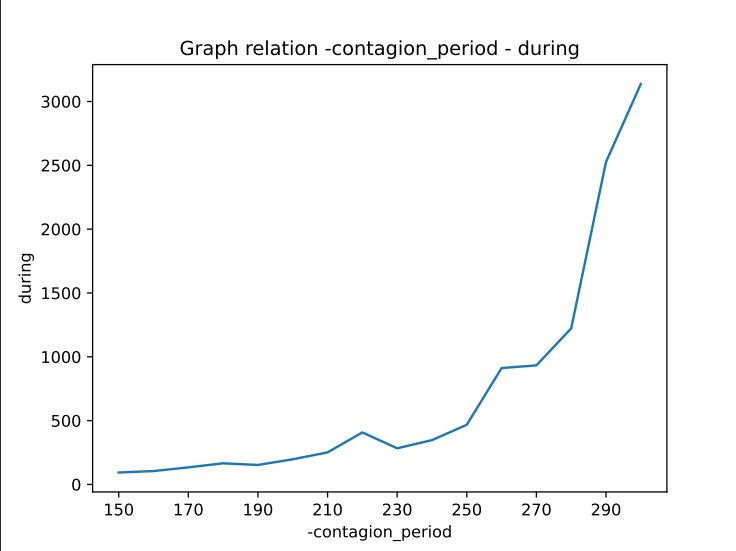
\includegraphics[scale=0.45]{attachements/contagion_period_during.png}
				
				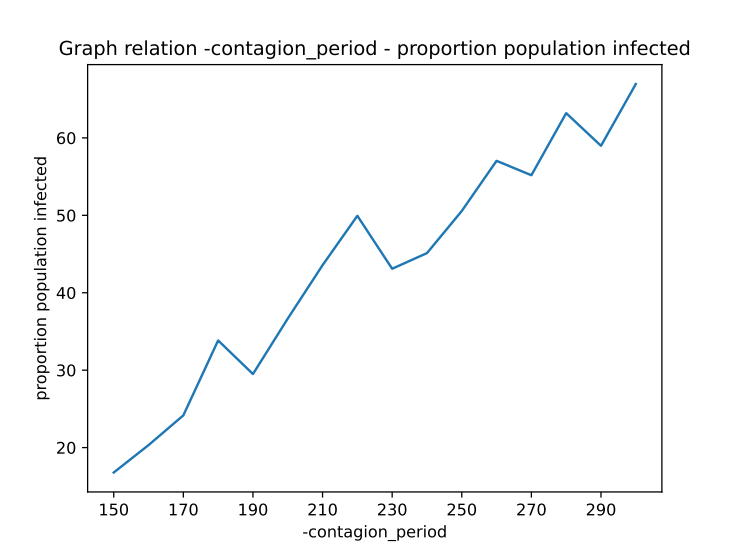
\includegraphics[scale=0.45]{attachements/contagion_period_proportion.png}
				
				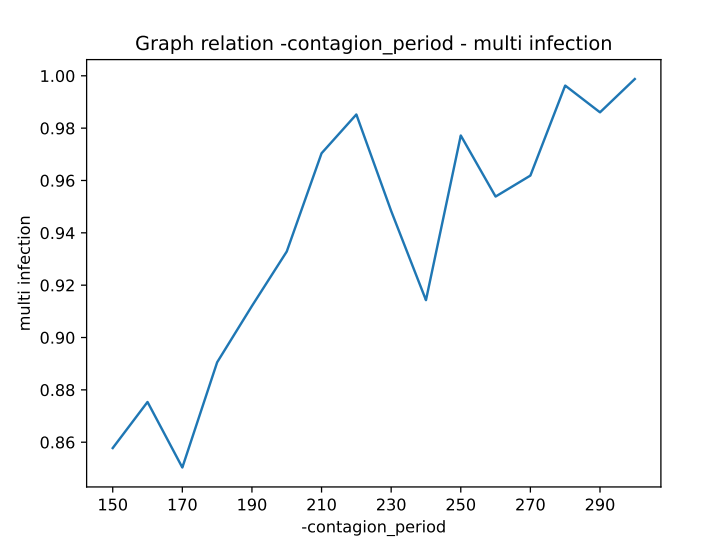
\includegraphics[scale=0.45]{attachements/contagion_period_multi_infection.png}
				
				
				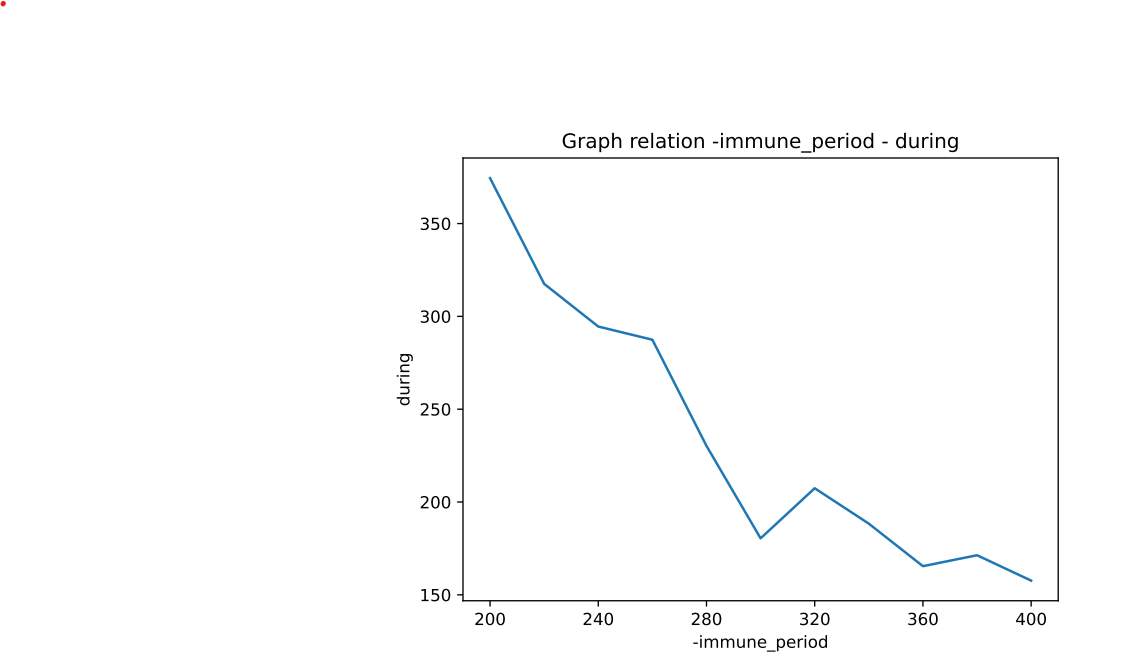
\includegraphics[scale=0.45]{attachements/immune_period_during.png}
				
				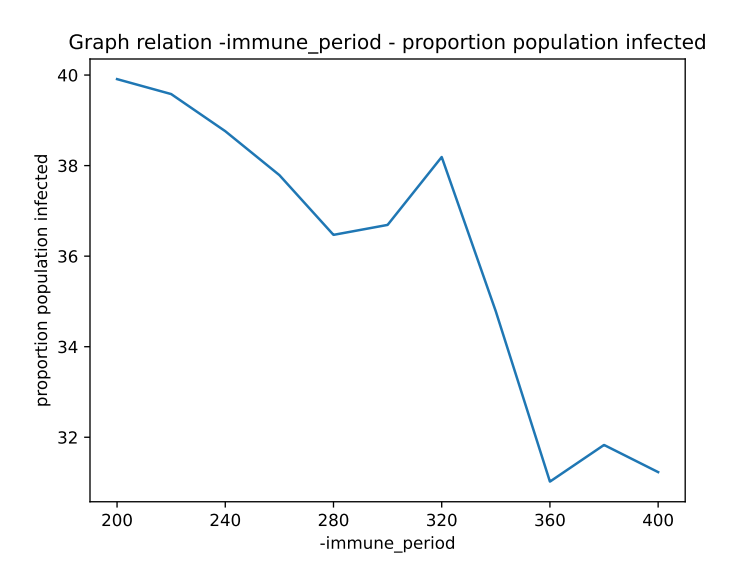
\includegraphics[scale=0.45]{attachements/immune_period_proportion.png}
				
				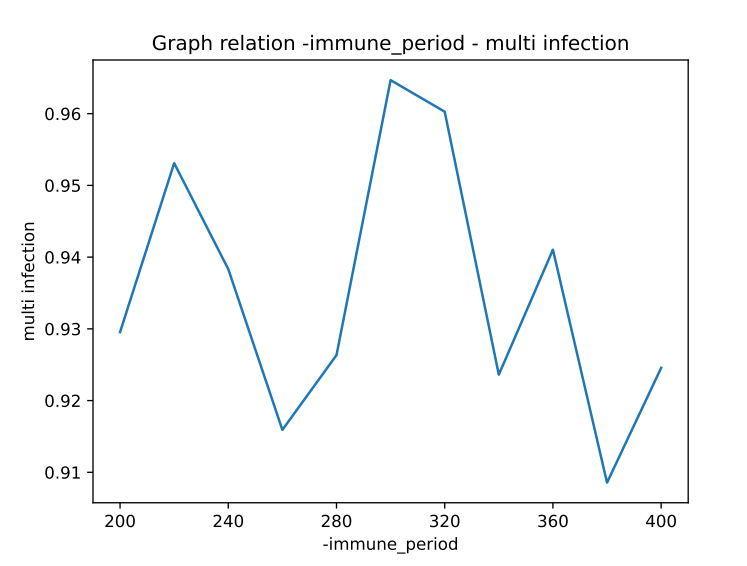
\includegraphics[scale=0.45]{attachements/immune_period_multi_infection.png}
				
				
				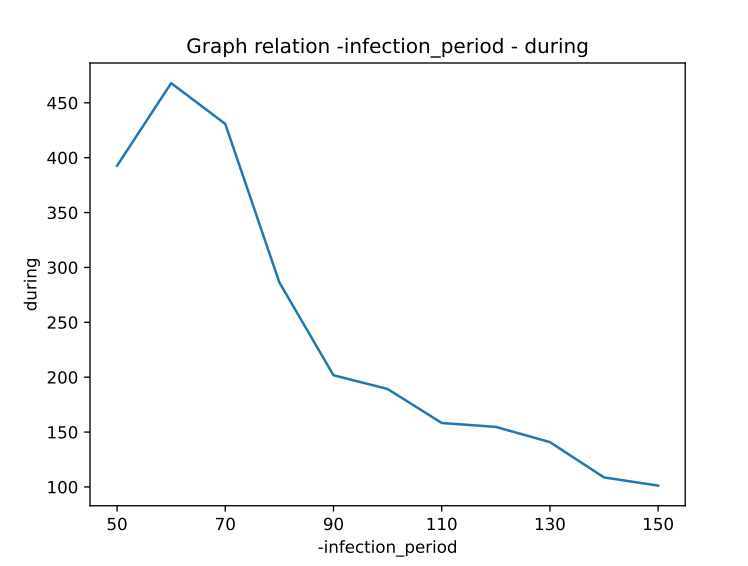
\includegraphics[scale=0.45]{attachements/infection_period_during.png}
				
				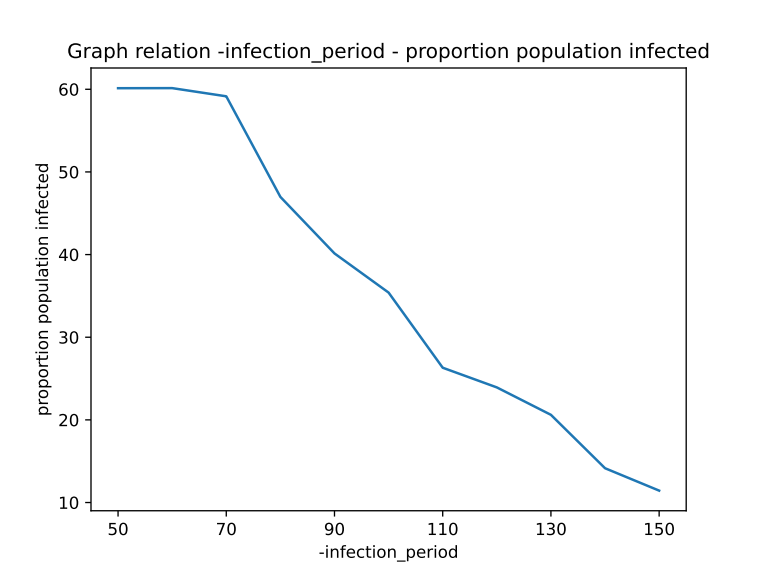
\includegraphics[scale=0.45]{attachements/infection_period_proportion.png}
				
				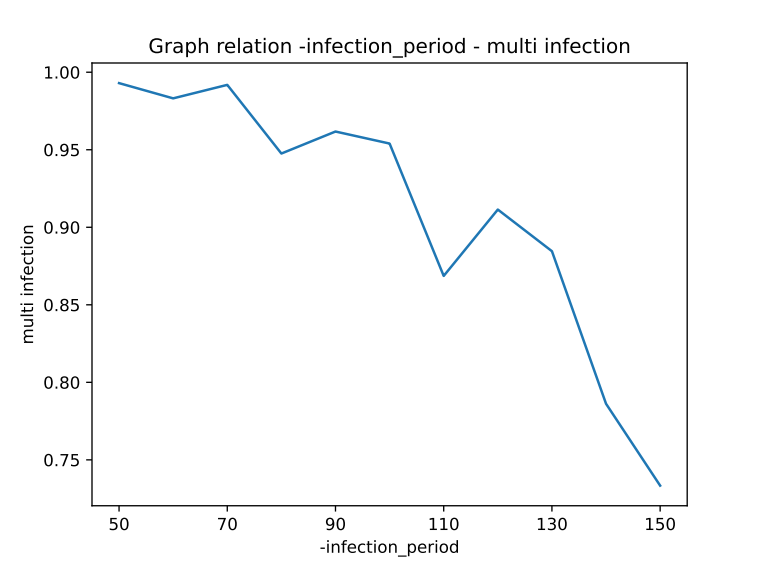
\includegraphics[scale=0.45]{attachements/infection_period_multi_infection.png}
				
				
				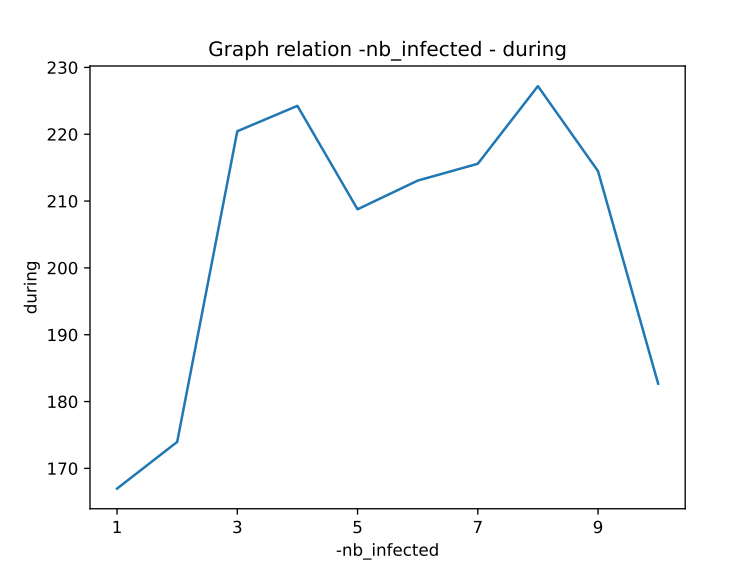
\includegraphics[scale=0.45]{attachements/nb_infected_during.png}
				
				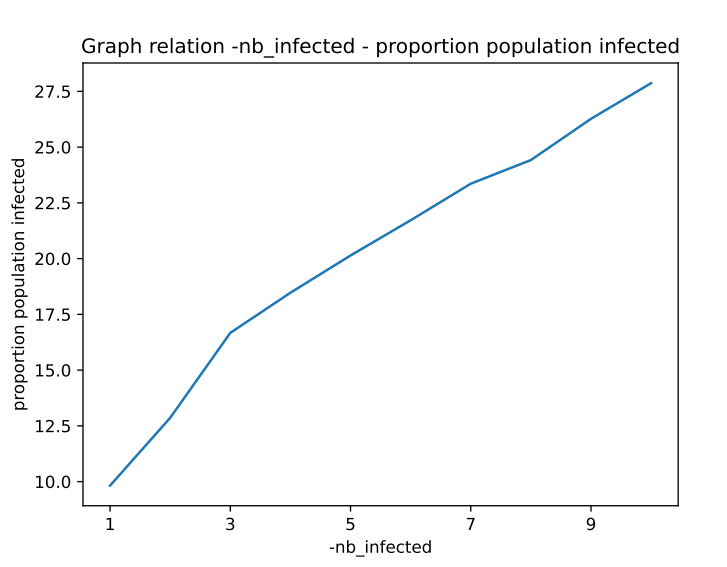
\includegraphics[scale=0.45]{attachements/nb_infected_proportion.png}
				
				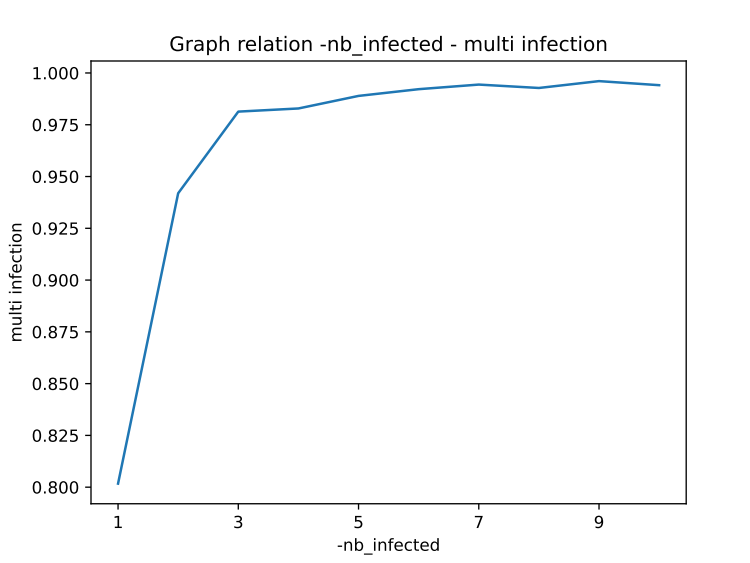
\includegraphics[scale=0.45]{attachements/nb_infected_multi_infection.png}
				
				
				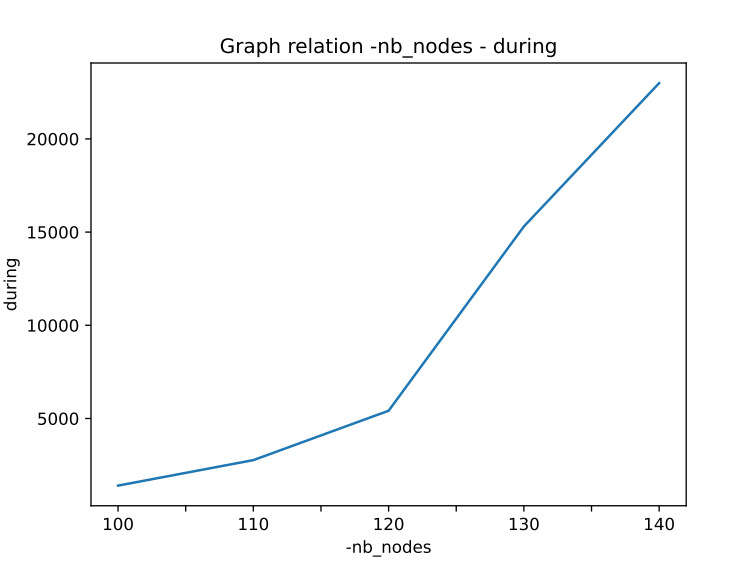
\includegraphics[scale=0.45]{attachements/nb_nodes_during.png}
				
				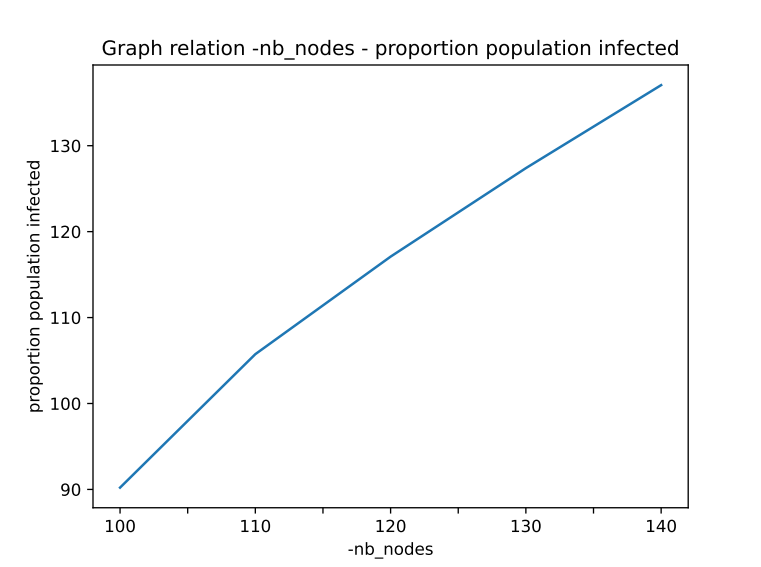
\includegraphics[scale=0.45]{attachements/nb_nodes_proportion.png}
				
				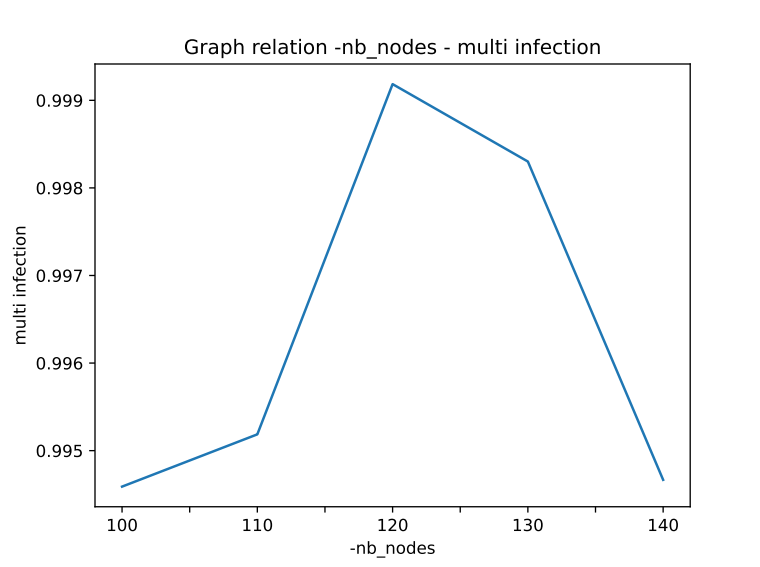
\includegraphics[scale=0.45]{attachements/nb_nodes_multi_infection.png}
				
				
				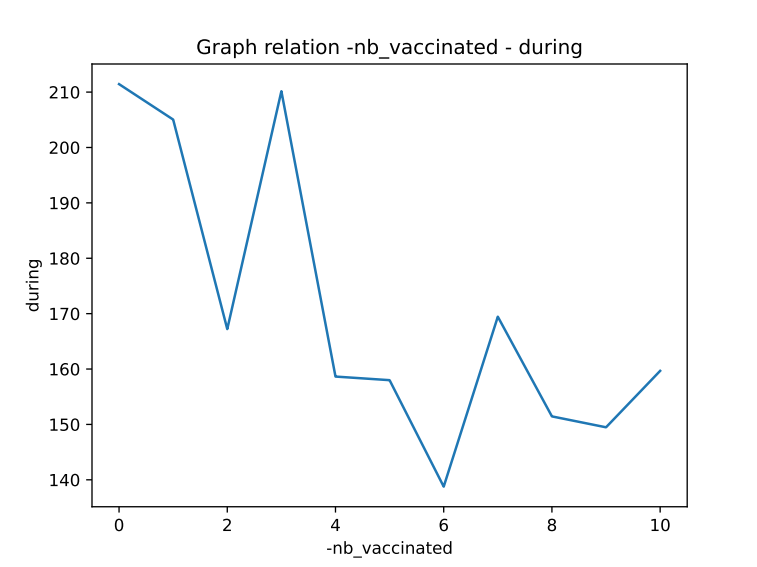
\includegraphics[scale=0.45]{attachements/nb_vaccinated_during.png}
				
				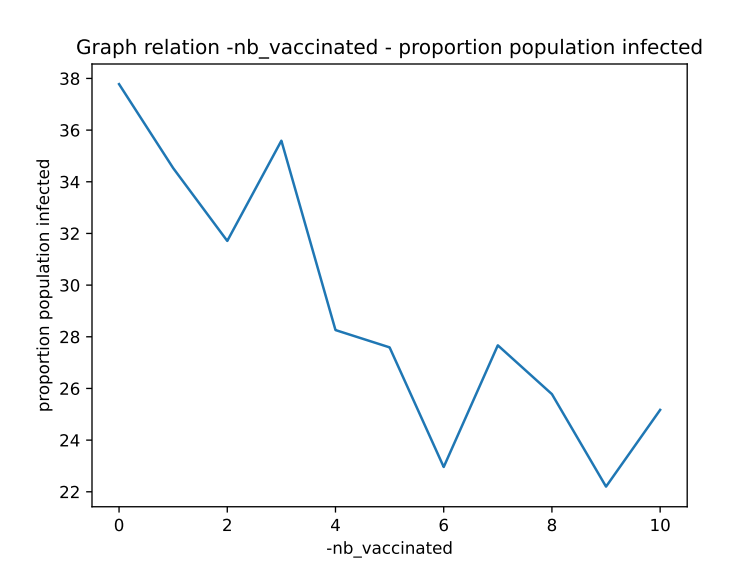
\includegraphics[scale=0.45]{attachements/nb_vaccinated_proportion.png}
				
				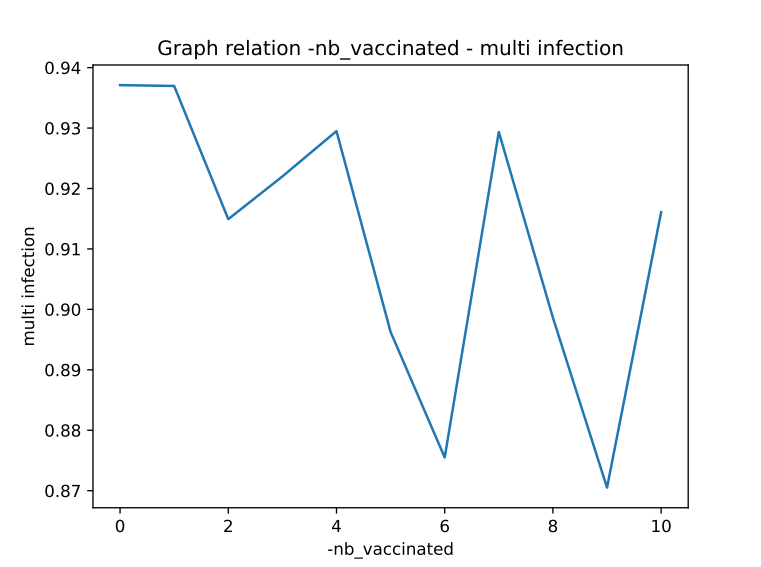
\includegraphics[scale=0.45]{attachements/nb_vaccinated_multi_infection.png}
				
				
				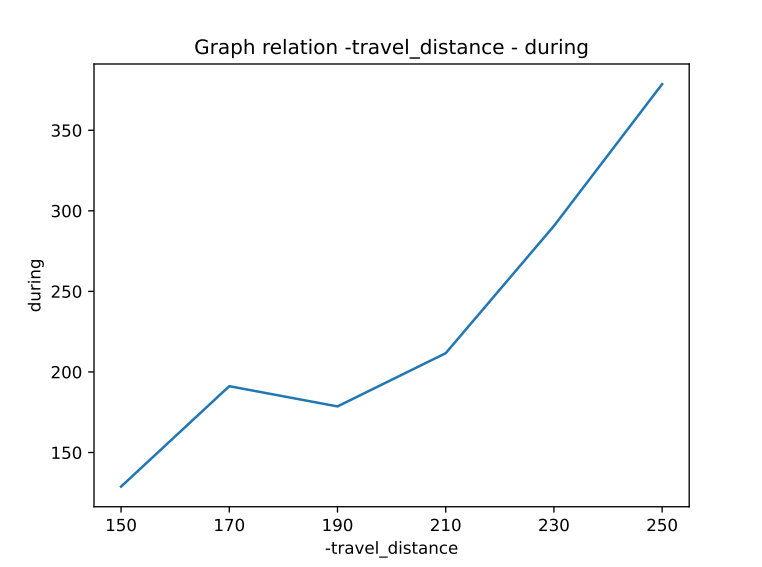
\includegraphics[scale=0.45]{attachements/travel_distance_during.png}
				
				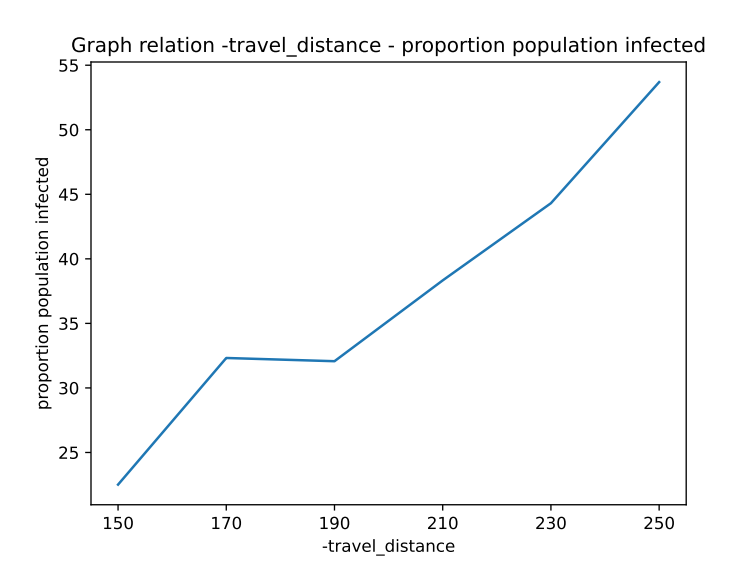
\includegraphics[scale=0.45]{attachements/travel_distance_proportion.png}
				
				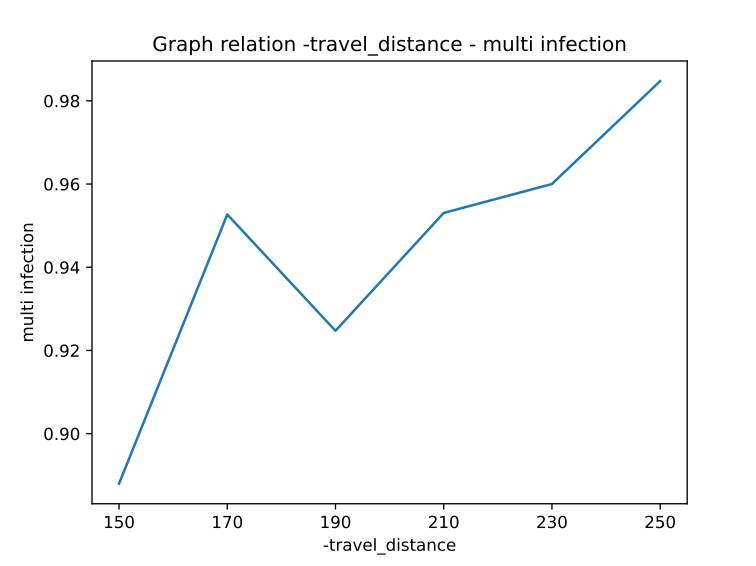
\includegraphics[scale=0.45]{attachements/travel_distance_multi_infection.png}
				
				
				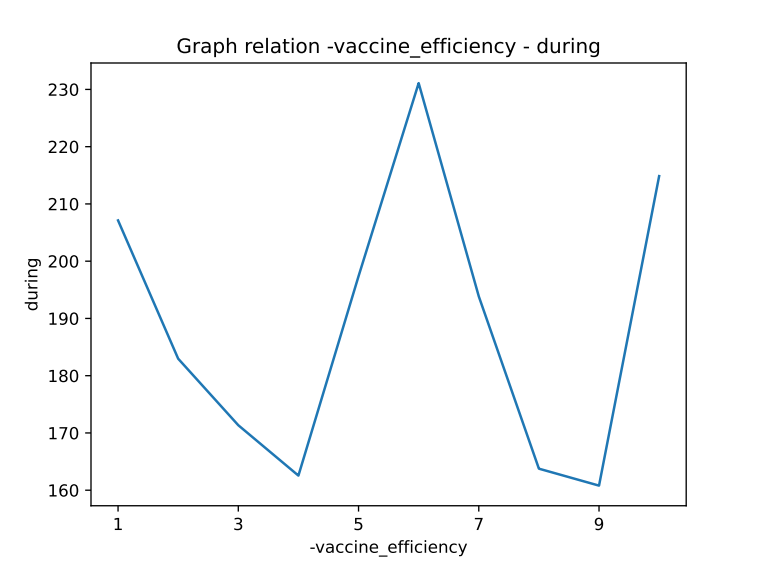
\includegraphics[scale=0.45]{attachements/vaccine_efficiency_during.png}
				
				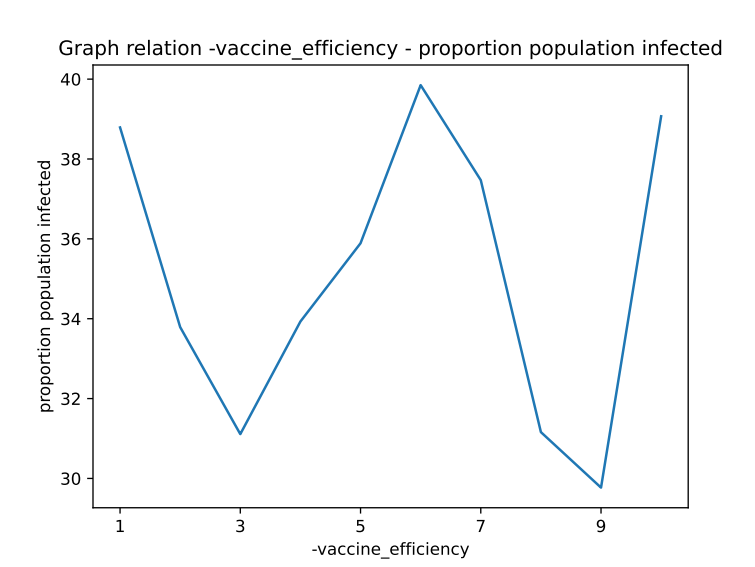
\includegraphics[scale=0.45]{attachements/vaccine_efficiency_proportion.png}
				
				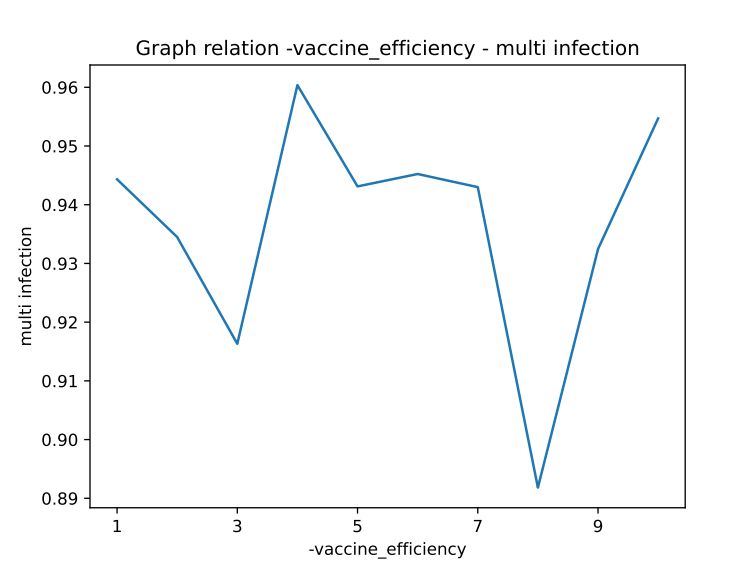
\includegraphics[scale=0.45]{attachements/vaccine_efficiency_multi_infection.png}
			% \end{multicols}


		\subsection{Enregistrement des résultats}
			
			Les résultats ainsi obtenus (tableaux et graph) sont sauvegardés dans des fichiers:
			\begin{itemize}
				\item nb\_infected:
				\begin{itemize}
					\item dossier: result\_analyse/nb\_infected
					\item durée: infected\_during.csv et infected\_during.pdf
					\item proportion population infected: infected\_proportion.csv et infected\_proportion.pdf
					\item multi infection: infected\_multi\_infection.csv et infected\_multi\_infection.pdf
				\end{itemize}
				
				\item travel\_distance:
				\begin{itemize}
					\item dossier: result\_analyse/travel\_distance
					\item durée: travel\_distance\_during.csv et travel\_distance\_during.pdf
					\item proportion population infected: travel\_distance\_proportion.csv et travel\_distance\_proportion.pdf
					\item multi infection: travel\_distance\_multi\_infection.csv et travel\_distance\_multi\_infection.pdf
				\end{itemize}
				
				\item nb\_vaccinated:
				\begin{itemize}
					\item dossier: result\_analyse/nb\_vaccinated
					\item durée: vaccinated\_during.csv et vaccinated\_during.pdf
					\item proportion population infected: vaccinated\_proportion.csv et vaccinated\_proportion.pdf
					\item multi infection: vaccinated\_multi\_infection.csv et vaccinated\_multi\_infection.pdf
				\end{itemize}
				
				\item vaccine\_efficiency:
				\begin{itemize}
					\item dossier: result\_analyse/vaccine\_efficiency
					\item durée: vaccine\_efficiency\_during.csv et vaccine\_efficiency\_during.pdf
					\item proportion population infected: vaccine\_efficiency\_proportion.csv et vaccine\_efficiency\_proportion.pdf
					\item multi infection: vaccine\_efficiency\_multi\_infection.csv et vaccine\_efficiency\_multi\_infection.pdf
				\end{itemize}
				
				\item infection\_period:
				\begin{itemize}
					\item dossier: result\_analyse/infection\_period
					\item durée: infection\_period\_during.csv et infection\_period\_during.pdf
					\item proportion population infected: infection\_period\_proportion.csv et infection\_period\_proportion.pdf
					\item multi infection: infection\_period\_multi\_infection.csv et infection\_period\_multi\_infection.pdf
				\end{itemize}
				
				\item contagion\_period:
				\begin{itemize}
					\item dossier: result\_analyse/contagion\_period
					\item durée: contagion\_period\_during.csv et contagion\_period\_during.pdf
					\item proportion population infected: contagion\_period\_proportion.csv et contagion\_period\_proportion.pdf
					\item multi infection: contagion\_period\_multi\_infection.csv et contagion\_period\_multi\_infection.pdf
				\end{itemize}
				
				\item immune\_period:
				\begin{itemize}
					\item dossier: result\_analyse/immune\_period
					\item durée: immune\_period\_during.csv et immune\_period\_during.pdf
					\item proportion population infected: immune\_period\_proportion.csv et immune\_period\_proportion.pdf
					\item multi infection: immune\_period\_multi\_infection.csv et immune\_period\_multi\_infection.pdf
				\end{itemize}
				
				\item nb\_nodes:
				\begin{itemize}
					\item dossier: result\_analyse/nb\_nodes
					\item durée: nodes\_during.csv et nodes\_during.pdf
					\item proportion population infected: nodes\_proportion.csv et nodes\_proportion.pdf
					\item multi infection: nodes\_multi\_infection.csv et nodes\_multi\_infection.pdf
				\end{itemize}
			\end{itemize}
	
	\section{Liens utiles}
	
		\subsection{Lien vers la repository Github du projet}
		
		[projet gihbub](https://github.com/adrienKoumgangT/SimulationCampaignPython).
		
		\subsection{Lien vers la vidéo de présentation du projet}
		
		[video presentation mp3](https://drive.google.com/drive/folders/1dzkosGB8VdcnGMDaBYeceW4Zb-v5ZyTo?usp=sharing).
	
\end{document}